\documentclass{scrartcl}
\usepackage[utf8]{inputenc}
\usepackage[T1]{fontenc}
\usepackage[ngerman]{babel}
\usepackage{amssymb}
\usepackage{amsmath}
\usepackage{algorithmicx}
\usepackage{algpseudocode}
\usepackage{graphicx}
\usepackage{framed}
\usepackage{xcolor}
\usepackage[nottoc]{tocbibind}
\usepackage{caption}
\usepackage{setspace}
\onehalfspacing

\colorlet{shadecolor}{gray!25}
\setlength{\parindent}{0pt}

\newcommand{\abs}[1]{\left\lvert#1\right\rvert}
\newcommand{\R}{\mathbb{R}}

\begin{document}

\title{Lösen des Poisson-Problems mittels Finite-Differenzen-Diskretisierung\\
und LU-Zerlegung}
\author{Marisa Breßler und Anne Jeschke (PPI27)}
\date{03.01.2020}
\maketitle

\tableofcontents

\pagebreak
\section{Einleitende Worte}
In unserem Bericht  vom 29.11.2019 haben wir das Poisson-Problem vorgestellt und einen numerischen Lösungsansatz aufgezeigt, der es mittels einer Diskretisierung des Gebietes und des Laplace-Operators in das Lösen eines linearen Gleichungssystems überführt.
Letzteres soll nun wie angekündigt durchgeführt werden.
In dieser Arbeit wollen wir das lineare Gleichungssystem direkt lösen.
Dazu nutzen wir die LU-Zerlegung (mit Spalten- und Zeilenpivotisierung) der ermittelten tridiagonalen Block-Matrix $A^d$.

Anhand einer Beispielfunktion und den bereits im vorherigen Bericht betrachteten Fällen des Einheitsintervalls, -quadrates, -würfels (d.h. für das Gebiet $\Omega\subset\R^d$ ($d\in\mathbb{N}$) und dessen Rand $\partial\Omega$ gilt:
$\Omega=(0,1)^d$, $d\in\{1, 2, 3\}$ mit der Randbedingung $u \equiv 0$ auf $\partial\Omega$, wobei $u$ die gesuchte Funktion ist)
wollen wir im Folgenden die Funktionalität (Genauigkeit/Fehler, Konvergenzgeschwindigkeit, Effizienz) dieses Lösungsverfahrens exemplarisch untersuchen.
Alle im Rahmen dessen nötigen theoretischen Grundlagen finden sich in unseren vorherigen Berichten.

\pagebreak
\section{Untersuchungen zur Genauigkeit}
Für unsere Untersuchungen wählen wir die Beispielfunktion $u: \Omega \rightarrow \mathbb{R}$, die wie folgt definiert ist:
\[u(x) := \prod \limits_{l=1}^{d} x_l \, sin(\pi x_l)\]
Dabei sei wie bereits erwähnt $\Omega = (0,1)^d$ und $d\in\{1, 2, 3\}$.
Die Funktion $u$ ist die exakte Lösung des Poisson-Problems, sie wird in der Praxis gesucht. Bekannt ist lediglich die Funktion $f\in C(\Omega ; \R)$ und $\forall \, x \in\Omega$ gelte $-\Delta u(x) = f(x)$. Dementsprechend ist die Funktion $f: \Omega \rightarrow \mathbb{R}$ gegeben durch:
\[f(x) = ... \]

Die Genauigkeit unserer numerischen Lösung des Poisson-Problems -- wir nennen diese gesuchte Funktion $\hat{u}$ (denn sie ist die Approximation der exakten Lösungsfunktion $u$) -- ist abhängig von der Größenordnung der Fehler. Der Gesamtfehler setzt sich aus Verfahrens-/Approximationsfehler auf der einen und Rundungsfehler auf der anderen Seite zusammen\cite{tischendorf2019}. Im Folgenden wollen wir beide Fehlerarten in Hinblick auf unser Beispiel betrachten.

\subsection{Verfahrens-/Approximationsfehler}
Die Genauigkeit der berechneten numerischen Approximation wird höher,je mehr Diskretisierungspunkte man wählt, d.h. je größer die Anzahl der Intervalle $n$, bzw. je kleiner die Intervalllänge $h$ ist. Es gilt $h=n^{-1}$.

Dies wird im Folgenden beispielhaft für den Fall $d=2$ dargestellt.

{
  \centering
    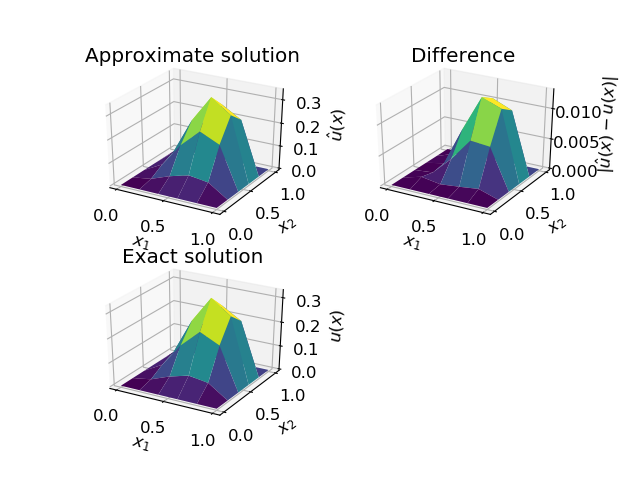
\includegraphics[width=0.75\textwidth]{Grafiken/3D_n=5}
    \vspace{-0.2cm}
    \captionof{figure}{Approximierte Lösung, exakte Lösung und deren absolute Differenz für $n = 5$}
    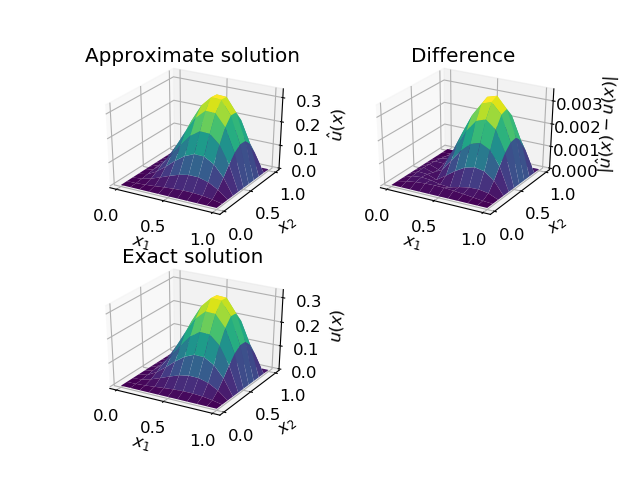
\includegraphics[width=0.75\textwidth]{Grafiken/3D_n=10}
    \vspace{-0.2cm}
    \captionof{figure}{Approximierte Lösung, exakte Lösung und deren absolute Differenz für $n = 10$}
    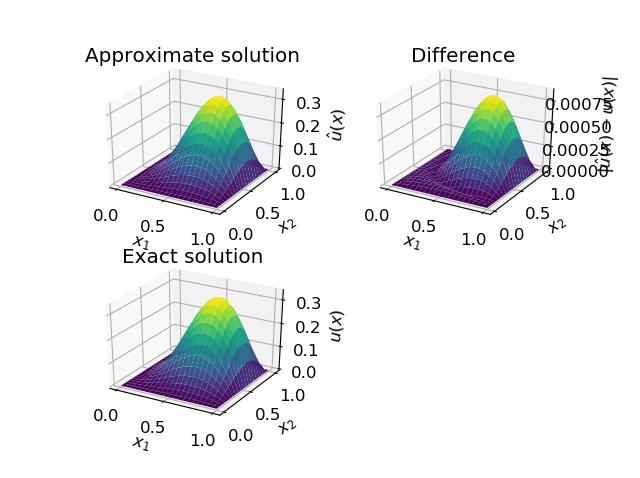
\includegraphics[width=0.75\textwidth]{Grafiken/3D_n=20}
    \vspace{-0.2cm}
    \captionof{figure}{Approximierte Lösung, exakte Lösung und deren absolute Differenz für $n = 20$}
}
\vspace{0.5cm}

Schon bei der sehr groben Diskretisierung mit $n=5$ kann man den Unterschied zwischen den beiden Lösungen mit bloßem Auge kaum erkennen, weshalb wir uns entschieden haben auch die absolute Differenz der beiden darzustellen.
Wie man dort sehen kann, erreicht man durch Erhöhung der Anzahl der Intervalle eine immer genauere Approximation der exakten Lösungsfunktion. Die absolute Differenz der Approximation und der exakten Lösung hält sich in einer immer kleineren Größenordnung auf.

{
  \centering
    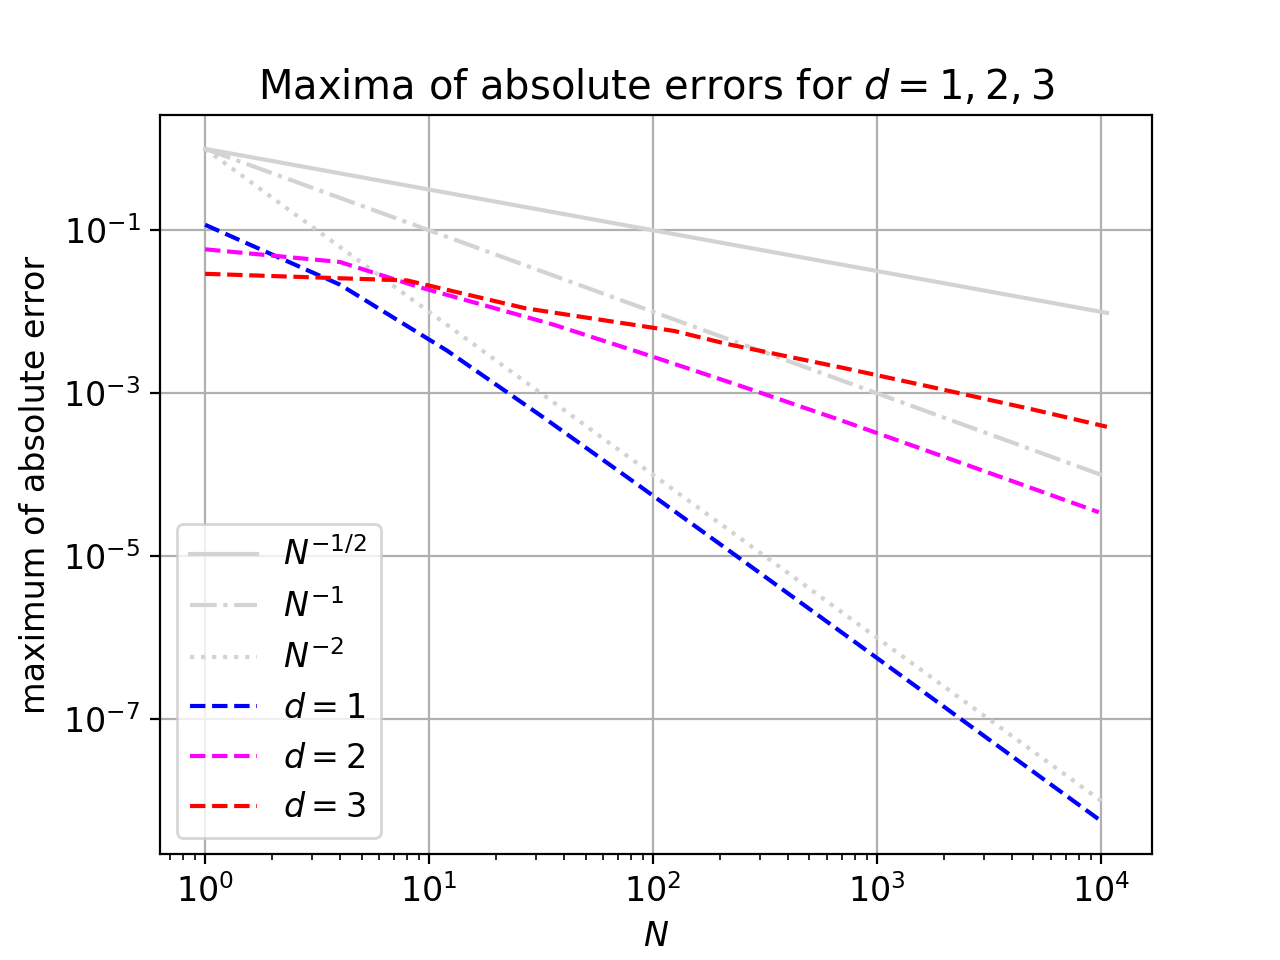
\includegraphics[width=0.75\textwidth]{Grafiken/loglogerr_d123_neu}
    \vspace{-0.2cm}
    \captionof{figure}{Konvergenzplot der maximalen Fehler in Abhängigkeit von $N$}
}
\vspace{0.5cm}

Man kann erkennen, dass mit größerem $N$, d.h. mit mehr Diskretisierugnspunkten, der Fehler immer kleiner wird, wobei er sich bei höheren Dimensionen langsamer verkleinert.
Für $d=1$ lässt sich in der Abbildung eine Konvergenzgeschwindigkeit von $N^{-2}$ erkennen. Für $d=2$ hingegen nur noch eine von $N^{-1}$ und bei $d=3$ von $N^{-1/2}$.

{
  \centering
    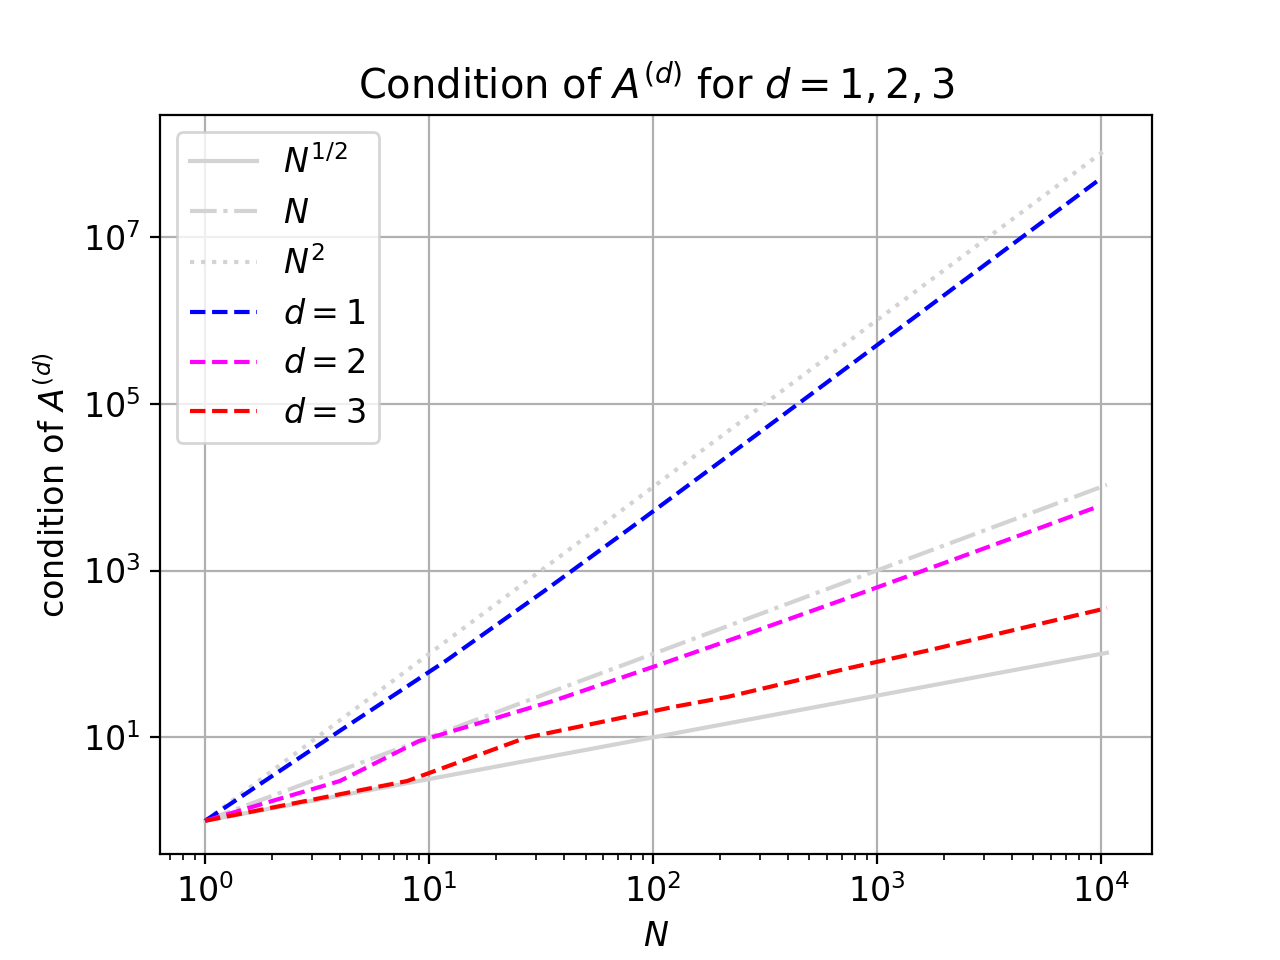
\includegraphics[width=0.75\textwidth]{Grafiken/loglogcond_d123_neu}
    \vspace{-0.2cm}
    \captionof{figure}{Konvergenzplot der maximalen Fehler in Abhängigkeit von $N$}
}
\vspace{0.5cm}

Konditionsplot von $A^d$ (1 Grafik)

\subsection{Rundungsfehler}
Lösen eines linearen Gleichungssystems beschreibt mathematisches Problem

Kondition einer Matrix: Maß für Abhängigkeit der Lösung eines Problems von Störung der Eingangsdaten

Konditionszahl: Faktor, um den sich der Eingangsfehler maximal verstärken kann

Vgl. Kondition von $A^d$ und der entsprechenden Hilbertmatrix mit gleicher Dimension (Tabelle)

\pagebreak
\section{Untersuchungen zum Speicherplatz}
sparsity von $A^d$ und deren LU-Zerlegung (3 Grafiken)

\pagebreak
\section{Zusammenfassung und Ausblick}


\pagebreak

\bibliographystyle{plain}
\bibliography{serie3_literatur}

\end{document}